
 \begin{figure}[ht]
 	\centerline{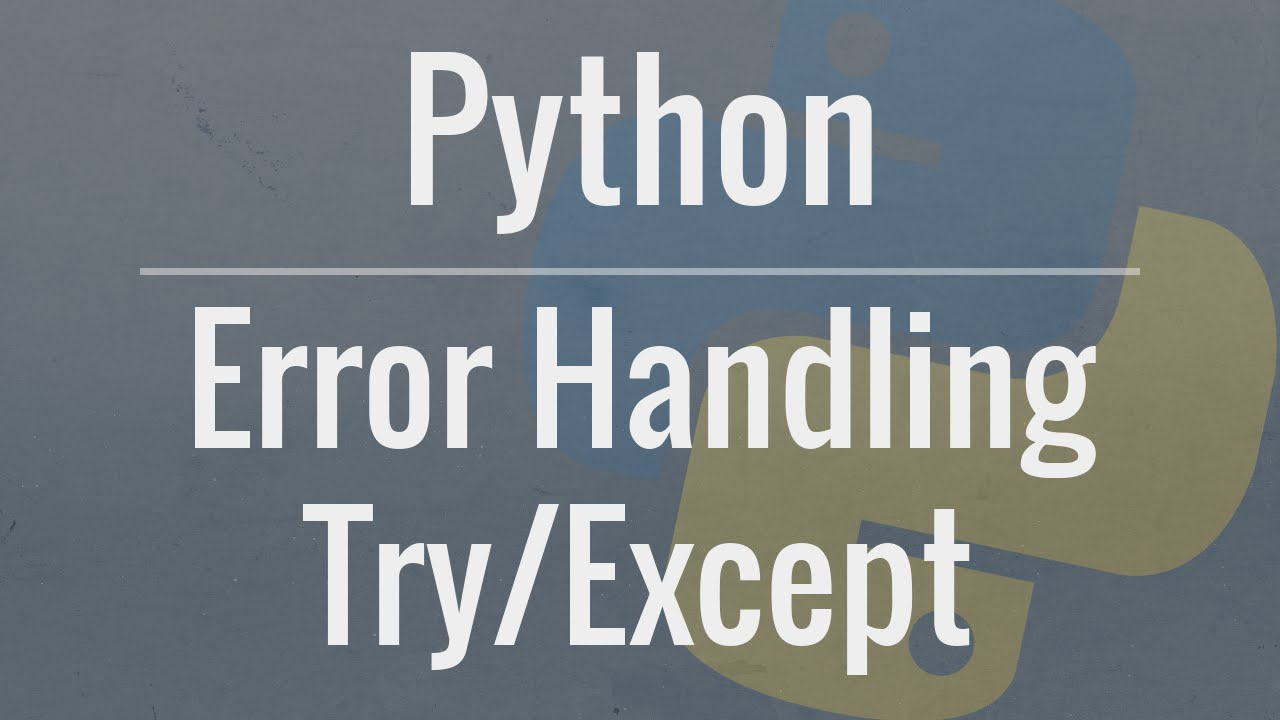
\includegraphics[width=0.60\textwidth]{Gambar/dapi6.jpg}}
 	\caption{Python Exceptions Handling}
 	\label{Python Exceptions Handling}
 \end{figure}
 
 
 
 \section {Pengertian }
 \subsection {Python Exceptions Handling}
 
 
 \hspace*{0.64in} Python menyediakan dua fitur yang sangat penting untuk menangani kesalahan tak terduga dalam program Python Anda dan menambahkan kemampuan debugging di dalamnya Exception Handling: Ini akan dibahas dalam tutorial ini. Berikut adalah daftar standar Pengecualian yang tersedia dengan Python: Pengecualian Standar. Penegasan: Ini akan dibahas dalam Asertions dengan tutorial Python. Daftar Pengecualian Standar – Penegasan dengan Python Penegasan adalah pemeriksaan kewarasan yang dapat Anda aktifkan atau matikan saat Anda selesai dengan pengujian program Anda. Cara termudah untuk memikirkan sebuah pernyataan adalah menyamakannya dengan pernyataan kenaikan gaji-jika (atau lebih akurat, pernyataan kenaikan-jika-tidak). Sebuah ekspresi diuji, dan jika hasilnya muncul salah, pengecualian akan meningkat. Penegasan dilakukan dengan pernyataan tegas, kata kunci terbaru untuk Python, diperkenalkan di versi 1.5. Pemrogram sering menempatkan asersi pada awal fungsi untuk memeriksa masukan yang valid, dan setelah pemanggilan fungsi untuk memeriksa keluaran yang valid. Pernyataan tegas Ketika menemukan pernyataan tegas, Python mengevaluasi ekspresi yang menyertainya, yang semoga benar. Jika ungkapannya salah, Python menimbulkan pengecualian AssertionError. Sintaks untuk menegaskan adalah -menegaskan Ekspresi [, Argumen]. 
 
 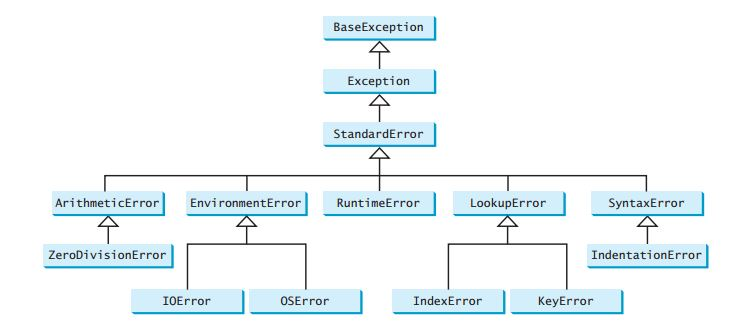
\includegraphics[width=15cm,height=7cm]{Gambar/dapi5.jpg}
 \begin{equation}Python Exceptions Handling\end{equation}
 

\section{Kelas dasar untuk semua pengecualian } 

\subsection{EXCEPTION NAME }

\vspace{12pt}
 \begin{enumerate}
\item StopIteration 

Dibesarkan ketika metode (iterator) berikutnya dari iterator tidak mengarah ke objek apa pun. 
\vspace{12pt}

\item SystemExit 
Dibesarkan oleh fungsi sys.exit () 
\vspace{12pt}

\item StandardError 
 
Kelas dasar untuk semua pengecualian built-in kecuali StopIteration dan SystemExit 
\vspace{12pt}

\item ArithmeticError 
 
Kelas dasar untuk semua kesalahan yang terjadi untuk perhitungan numerik. 
\vspace{12pt}

\item OverflowError 

Dibesarkan saat perhitungan melebihi batas maksimum untuk tipe numerik.
\vspace{12pt}

\item FloatingPointError   

Dibesarkan saat perhitungan floating point gagal. 
\vspace{12pt}

\item ZeroDivisionError  

Dibesarkan saat pembagian atau modulo nol dilakukan untuk semua tipe numerik. 
\vspace{12pt}
\vspace{12pt}

\item AssertionError 

Dibesarkan jika terjadi kegagalan pernyataan Assert. 
\vspace{12pt}

\item AttributeError 
 
Dibesarkan jika terjadi kegagalan referensi atribut atau penugasan.
\vspace{12pt}

\item EOFError 

Dibesarkan bila tidak ada input dari fungsi raw $  \_  $input () atau input () dan akhir file tercapai. 
\vspace{12pt}

\item ImportError 

Dibesarkan saat sebuah pernyataan impor gagal. 
\vspace{12pt}

\item KeyboardInterrupt  

Dibesarkan saat pengguna menyela eksekusi program, biasanya dengan menekan Ctrl + c. 
\vspace{12pt}

\item LookupError  

Kelas dasar untuk semua kesalahan pencarian. 
\vspace{12pt}


\item KeyError 
 
Dibesarkan saat sebuah indeks tidak ditemukan secara berurutan. Dibesarkan saat kunci yang ditentukan tidak ditemukan dalam kamus. 
\vspace{12pt}

\item NameError 

Dibesarkan saat pengenal tidak ditemukan di namespace lokal atau global. 
\vspace{12pt}



\item EnvironmentError  
 
Dibesarkan saat mencoba mengakses variabel lokal dalam suatu fungsi atau metode namun tidak nilai yang ditugaskan padanya. Kelas dasar untuk semua pengecualian yang terjadi di luar lingkungan Python. 
\vspace{12pt}


\item IOError 

IOError Dibesarkan saat operasi input / output gagal, seperti pernyataan cetak atau fungsi open () saat mencoba membuka file yang tidak ada. Dibangkitkan untuk kesalahan terkait sistem operasi. 
\vspace{12pt}

\end {enumerate}
 
\section{SyntaxError} 

\begin{enumerate}


\item IndentationError 

Dibesarkan saat ada kesalahan dengan sintaks Python. Dibesarkan saat indentasi tidak ditentukan dengan benar. 


\item SystemError  

Dibesarkan saat penafsir menemukan masalah internal, namun bila kesalahan ini ditemui juru bahasa Python tidak keluar. 
\vspace{12pt}




\item SystemExit  

Dibesarkan saat juru bahasa Python berhenti dengan menggunakan fungsi sys.exit (). Jika tidak ditangani dalam kode, menyebabkan penafsir untuk keluar. 
\vspace{12pt}


\item TypeError 

Dibesarkan saat operasi atau fungsi dicoba yang tidak valid untuk tipe data yang ditentukan. 
\vspace{12pt}


\item ValueError 

Dibesarkan saat fungsi bawaan untuk tipe data memiliki jenis argumen yang valid, namun argumen tersebut memiliki nilai yang tidak valid yang ditentukan. 
\vspace{12pt}

\item RuntimeError 

Dibesarkan saat kesalahan yang dihasilkan tidak termasuk dalam kategori apa pun. 
\vspace{12pt}

 \end {enumerate}

 \hspace*{0.5in} Jika asersi gagal, Python menggunakan ArgumentExpression sebagai argumen untuk AssertionError. Penegasan Pengecualian pengecualian dapat ditangkap dan ditangani seperti pengecualian lainnya dengan menggunakan perintah try-except, namun jika tidak ditangani, mereka akan menghentikan program dan menghasilkan traceback. 
 
Contoh Berikut adalah fungsi yang mengubah suhu dari derajat Kelvin sampai derajat Fahrenheit. Karena nol derajat Kelvin sedingin yang didapatnya, fungsi itu mundur jika melihat suhu negatif –
\vspace{12pt}
\begin{verbatim}
 $  \#  $!/usr/bin/python 
 
def KelvinToFahrenheit(Temperature): 

~~ assert (Temperature >= 0),"Colder than absolute zero!" 

~~ return ((Temperature-273)*1.8)+32 

print KelvinToFahrenheit(273) 

print int(KelvinToFahrenheit(505.78)) 

print KelvinToFahrenheit(-5) 
\vspace{14pt}

Bila kode diatas dieksekusi, maka menghasilkan hasil sebagai berikut – 
\vspace{12pt}

32.0 

451 

Traceback (most recent call last): 

File "test.py", line 9, in  

print KelvinToFahrenheit(-5) 

File "test.py", line 4, in KelvinToFahrenheit

assert (Temperature >= 0),"Colder than absolute zero!" 

AssertionError: Colder than absolute zero! 
\vspace{12pt}
\end{verbatim}
Apa itu Exception? 

Pengecualian adalah sebuah peristiwa, yang terjadi selama pelaksanaan program yang mengganggu aliran normal instruksi program. Secara umum, ketika skrip Python menemukan situasi yang tidak dapat diatasi, hal itu menimbulkan pengecualian. Pengecualian adalah objek Python yang mewakili kesalahan. 
\vspace{12pt}

Ketika skrip Python menimbulkan pengecualian, ia harus menangani pengecualian begitu saja sehingga berhenti dan berhenti. Menangani pengecualian Jika Anda memiliki beberapa kode yang mencurigakan yang mungkin menimbulkan pengecualian, Anda dapat mempertahankan program Anda dengan menempatkan kode yang mencurigakan di coba: blokir. Setelah dicoba: blokir, sertakan sebuah pernyataan kecuali:, diikuti oleh blok kode yang menangani masalah ini seaman mungkin. Sintaksis Berikut adalah sintaks sederhana coba .... kecuali ... blok lain – 
\vspace{12pt}

\begin{verbatim}
try: 

~~ You do your operations here; 

~~ ...................... 

except \textit{ExceptionI}: 

~~ If there is ExceptionI, then execute this block. 

except \textit{ExceptionII}: 

~~ If there is ExceptionII, then execute this block. 

~~ ...................... 

else: 

~~ If there is no exception then execute this block 
\vspace{12pt}
\vspace{12pt}

\end{verbatim}

Berikut adalah beberapa poin penting tentang sintaks yang disebutkan di atas - 

 \hspace*{0.5in} \vspace{12pt}
\vspace{12pt}

 \hspace*{0.5in} Pernyataan percobaan tunggal dapat memiliki banyak kecuali pernyataan. Ini berguna saat blok coba berisi pernyataan yang mungkin membuang berbagai jenis pengecualian. $  $Anda juga bisa memberikan klausa umum kecuali klausul, yang menangani pengecualian apapun.Setelah klausa kecuali, Anda bisa memasukkan klausul lain. Kode di blok yang lain dijalankan jika kode di coba: blok tidak menimbulkan pengecualian.Blok yang lain adalah tempat yang baik untuk kode yang tidak perlu dicoba: perlindungan blokir. Contoh Contoh ini membuka file, menulis konten di file, dan keluar dengan anggun karena tidak ada masalah sama sekali - 
\vspace{16pt}

\begin{verbatim}

 $  \#  $!/usr/bin/python 
\vspace{12pt}
 
try: 

~~ fh = open("testfile", "w") 

~~ fh.write("This is my test file for exception handling!!") 

except IOError: 

~~ print "Error: can $  \setminus  $'t find file or read data" 

else: 

~~ print "Written content in the file successfully" 

~~ fh.close() 
\vspace{16pt}

Ini menghasilkan hasil sebagai berikut - 
\vspace{12pt}

Written content in the file successfully 
\vspace{12pt}
 
 \end{verbatim}
 
Klausul kecuali tanpa pengecualian anda juga dapat menggunakan pernyataan kecuali tanpa pengecualian yang didefinisikan sebagai berikut - 
\vspace{12pt}

\begin{verbatim}

try: 

~~ You do your operations here; 

~~ ...................... 

except:

~~ If there is any exception, then execute this block. 

~~ ...................... 

else: 

~~ If there is no exception then execute this block.  
\vspace{12pt}
\vspace{16pt}

\end{verbatim}

 \hspace*{0.5in} Pernyataan try-except semacam ini menangkap semua pengecualian yang terjadi. Dengan menggunakan jenis try-except statement ini tidak dianggap sebagai praktik pemrograman yang bagus, karena menangkap semua pengecualian namun tidak membuat programmer mengenali akar permasalahan yang mungkin terjadi. Klausul Kecuali dengan Beberapa Pengecualian Anda juga dapat menggunakan pernyataan kecuali yang sama untuk menangani beberapa pengecualian sebagai berikut - 
\vspace{12pt}
 
try: 

~~ You do your operations here; 

~~ ...................... 

except(Exception1[, Exception2[,...ExceptionN]]]): 

~~ If there is any exception from the given exception list,  

~~ then execute this block. 

~~ ...................... 

else: 

~~ If there is no exception then execute this block.  
\vspace{12pt}
\vspace{12pt}
 
 $  \#  $!/usr/bin/python 
\vspace{12pt}

try: 

~~ fh = open("testfile", "w") 

~~ fh.write("This is my test file for exception handling!!") 
 
finally: 

~~ print "Error: can $  \setminus  $'t find file or read data" 
\vspace{12pt}
\vspace{12pt}
 
 $  \#  $!/usr/bin/python 
\vspace{12pt}
 
try: 

~~ fh = open("testfile", "w") 

~~ try: 
 
~~~~~ fh.write("This is my test file for exception handling!!") 

~~ finally: 

~~~~~ print "Going to close the file" 

~~~~~ fh.close() 

except IOError: 

~~ print "Error: can $  \setminus  $'t find file or read data" 
\vspace{12pt}
\vspace{16pt}

 \hspace*{0.5in} Bila dikecualikan dilempar di blok coba, eksekusi langsung lolos ke blok akhirnya. Setelah semua pernyataan di blok akhirnya dieksekusi, pengecualian dinaikkan lagi dan ditangani dalam pernyataan kecuali jika ada di lapisan yang lebih tinggi dari pernyataan try-except. Argumen Eksepsi Pengecualian dapat memiliki argumen, yang merupakan nilai yang memberi informasi tambahan tentang masalah tersebut. Isi argumen bervariasi menurut pengecualian. Anda menangkap argumen pengecualian dengan menyediakan sebuah variabel dalam klausa kecuali sebagai berikut - 
\vspace{12pt}

try: 

~~ You do your operations here;

~~ ...................... 

except \textit{ExceptionType}\textit{,}\textit{ }\textit{Argument}: 

~~ You can print value of Argument here... 
\vspace{12pt}

 \hspace*{0.5in} Jika Anda menulis kode untuk menangani satu pengecualian, Anda dapat memiliki variabel mengikuti nama pengecualian dalam pernyataan kecuali. Jika Anda menjebak beberapa pengecualian, Anda dapat memiliki variabel mengikuti tuple pengecualian. Variabel ini menerima nilai pengecualian yang sebagian besar mengandung penyebab pengecualian. Variabel tersebut dapat menerima satu nilai atau beberapa nilai dalam bentuk tuple. Tuple ini biasanya berisi error string, error number, dan error location. Pengecualian yang Ditentukan Pengguna Python juga memungkinkan Anda membuat pengecualian sendiri dengan menurunkan kelas dari pengecualian standar built-in. Berikut adalah contoh yang berkaitan dengan RuntimeError. Di sini, sebuah kelas dibuat yang dikelompokkan dari RuntimeError. Ini berguna saat Anda perlu menampilkan informasi yang lebih spesifik saat pengecualian tertangkap. Di blok percobaan, pengecualian yang ditentukan pengguna dinaikkan dan ditangkap di blok kecuali. Variabel e digunakan untuk membuat sebuah instance dari class Networkerror. 
\vspace{12pt}

{\fontsize{10pt}{10pt}\selectfont  (x,y) = (5,0)} 

{\fontsize{10pt}{10pt}\selectfont  try:} 

{\fontsize{10pt}{10pt}\selectfont ~~ z = x/y} 


{\fontsize{10pt}{10pt}\selectfont  except ZeroDivisionError:}


{\fontsize{10pt}{10pt}\selectfont ~~ print "divide by zero"} 

\vspace{10pt}

Jika Anda ingin memeriksa pengecualian dari kode, Anda bisa memiliki: 

\vspace{12pt}
 
\vspace{12pt}

\vspace{12pt}

{\fontsize{10pt}{10pt}\selectfont  (x,y) = (5,0)} 


{\fontsize{10pt}{10pt}\selectfont  try:} 


{\fontsize{10pt}{10pt}\selectfont ~~ z = x/y} 


{\fontsize{10pt}{10pt}\selectfont  except ZeroDivisionError as e:} 

{\fontsize{10pt}{10pt}\selectfont ~~ z = e  $  \#  $ representation: "<exceptions.ZeroDivisionError instance at 0x817426c>"} 


{\fontsize{10pt}{10pt}\selectfont  print z  $  \#  $ output: "integer division or modulo by zero"} 

\vspace{16pt}

General Error Catching 

\vspace{12pt}
 
 \hspace*{0.64in} Terkadang, Anda ingin menangkap semua kesalahan yang mungkin dihasilkan, tapi biasanya Anda tidak melakukannya. Dalam kebanyakan kasus, Anda ingin menjadi sespesifik mungkin (CatchWhatYouCanHandle). Pada contoh pertama di atas, jika Anda menggunakan klausul pengecualian catch-all dan pengguna menekan Ctrl-C, menghasilkan KeyboardInterrupt, Anda tidak ingin program mencetak "bagi dengan nol". Namun, ada beberapa situasi di mana yang terbaik untuk menangkap semua kesalahan. Misalnya, Anda menulis modul ekstensi ke layanan web. Anda ingin informasi kesalahan untuk output output halaman web, dan server untuk terus berjalan, jika mungkin. Tapi Anda tidak tahu kesalahan apa yang mungkin Anda masukkan ke dalam kode Anda. Dalam situasi seperti ini, Anda mungkin ingin mengode sesuatu seperti ini: 
\vspace{12pt}


{\fontsize{10pt}{10pt}\selectfont  import sys}
 

{\fontsize{10pt}{10pt}\selectfont  try:} 


{\fontsize{10pt}{10pt}\selectfont ~~ untrusted.execute()} 


{\fontsize{10pt}{10pt}\selectfont  except:  $  \#  $ catch *all* exceptions} 


{\fontsize{10pt}{10pt}\selectfont ~~ e = sys.exc $  \_  $info()[0]} 


{\fontsize{10pt}{10pt}\selectfont ~~ write $  \_  $to $  \_  $page( "<p>Error:  $  \%  $s</p>"  $  \%  $ e )} 
\vspace{10pt}

 \hspace*{0.64in} Menemukan Nama Pengecualian Spesifik Pengecualian standar yang dapat diajukan dijelaskan secara rinci pada: $  $
 Lihatlah dokumentasi kelas untuk mengetahui pengecualian apa yang bisa diberikan oleh kelas tertentu. Lihat juga: Di wiki ini: WritingExceptionClasses, TracebackModule. Untuk gagasan umum (non-Python specific) tentang pengecualian, berkonsultasilah dengan ExceptionPatterns. Untuk menulis tentang ... 

\vspace{12pt}
 
\begin{itemize}
\item Berikan contoh IOError, dan interpretasikan kode IOError. 

\item Berikan contoh beberapa pengecualian. Penanganan beberapa kecuali dalam satu baris.\end{itemize}
 
 
\vspace{12pt}

Pertanyaan Penanganan Kesalahan Umum, Di bagian "penanganan kesalahan umum" di atas, tertulis untuk menangkap semua pengecualian, Anda menggunakan kode berikut: 
\vspace{14pt}
 
{\fontsize{10pt}{10pt}\selectfont import sys} 


{\fontsize{10pt}{10pt}\selectfont  try:} 

\vspace{10pt}
 

{\fontsize{10pt}{10pt}\selectfont ~~ untrusted.execute()} 

\vspace{10pt}


{\fontsize{10pt}{10pt}\selectfont  except:  $  \#  $ catch *all* exceptions} 

\vspace{10pt}


{\fontsize{10pt}{10pt}\selectfont ~~ e = sys.exc $  \_  $info()[0]} 

\vspace{10pt}


{\fontsize{10pt}{10pt}\selectfont ~~ write $  \_  $to $  \_  $page( "<p>Error:  $  \%  $s</p>"  $  \%  $ e )} 
\vspace{16pt}


{\fontsize{10pt}{10pt}\selectfont  try:}

\vspace{10pt}
 
 
{\fontsize{10pt}{10pt}\selectfont ~~ untrusted.execute()} 

\vspace{10pt}

 
{\fontsize{10pt}{10pt}\selectfont  except Exception as e:} 

\vspace{10pt}

 
{\fontsize{10pt}{10pt}\selectfont ~~ write $  \_  $to $  \_  $page( "<p>Error:  $  \%  $s</p>"  $  \%  $ str(e) )} 
\vspace{16pt}

 \hspace*{0.64in} Seseorang menunjukkan bahwa "kecuali" menangkap lebih dari sekedar "kecuali Pengecualian sebagai e." Mengapa demikian? Apa bedanya? – LionKimbro Untuk saat ini (versi <= 2.4) pengecualian tidak harus diwarisi dari Exception. Jadi polos 'kecuali:'nangkap semua pengecualian, tidak hanya sistem. Pengecualian string adalah salah satu contoh pengecualian yang tidak mewarisi dari Exception. – MikeRovner Saya percaya bahwa pada 2,7, pengecualian masih tidak harus diwariskan dari Exception atau bahkan BaseException. Namun, seperti Python 3, pengecualian harus subclass BaseException. - gajah jim Mendapatkan Informasi Berguna dari Pengecualian Jadi, saya punya sesuatu seperti: 
 
\vspace{12pt}


{\fontsize{10pt}{10pt}\selectfont  (a,b,c) = d} 

\vspace{12pt}
 
dan Python kembali: 
 
\vspace{12pt}
 
 
{\fontsize{10pt}{10pt}\selectfont  ValueError: unpack list of wrong size} 
\vspace{16pt}

... dan begitulah, Anda tentu bertanya-tanya, "Nah, apa yang ada di d?" 

\vspace{12pt}

Anda tahu - Anda bisa mencetak di sana, dan itu berhasil. Tapi adakah cara yang lebih baik dan lebih menarik untuk mendapatkan informasi yang diketahui orang? Anda bisa melakukan sesuatu seperti: 
\vspace{20pt}

 
 try: 
 
 
~~ a, b, c = d 
 
 
 except Exception as e: 
 
 
~~ e.args += (d,) 
 
 
~~ raise 
\vspace{20pt}
 
 \hspace*{0.64in} Atribut .args pengecualian adalah tuple dari semua argumen yang dilewatkan (biasanya argumen satu dan satu-satunya adalah pesan kesalahannya). Dengan cara ini Anda dapat mengubah argumen dan menaikkan kembali, dan informasi tambahan akan ditampilkan. Anda juga bisa membuat pernyataan cetak atau login di blok kecuali. Perhatikan bahwa tidak semua pengecualian subclass Exception (meski hampir semua dilakukan), jadi ini mungkin tidak menangkap beberapa pengecualian; Selain itu, pengecualian tidak diperlukan untuk memiliki atribut .args (meskipun jika pengecualian subclass Exception dan tidak mengesampingkan  $  \_  $ $  \_  $init $  \_  $ $  \_  $ tanpa memanggil superclass-nya), maka kode yang ditulis mungkin gagal Namun dalam prakteknya hampir tidak pernah (dan Jika ya, Anda harus memperbaiki pengecualian yang tidak sesuai!) Bukankah lebih baik mencegahnya untuk melakukan remediasi? >  
 Joel Spolsky mungkin programmer hebat C ++, dan sarannya untuk desain antarmuka pengguna sangat berharga, tapi Python bukan C ++ atau Java, dan argumennya tentang pengecualian tidak berlaku dengan Python. Joel berpendapat: "Mereka tidak terlihat dalam kode sumber Melihat kumpulan kode, termasuk fungsi yang mungkin atau mungkin tidak membuang pengecualian, tidak ada cara untuk melihat pengecualian mana yang mungkin dilempar dan dari mana.Ini berarti bahwa pemeriksaan kode yang hati-hati pun tidak. Saya bisa mengungkapkan potensi bug. " 

 \hspace*{0.64in} (Perhatikan bahwa ini juga merupakan argumen di balik pengecualian yang diperiksa oleh Java - sekarang eksplisit bahwa pengecualian dapat dilemparkan - kecuali bahwa RuntimeException masih dapat dibuang ke mana saja. -jJ) Saya tidak mengerti argumen ini. Dalam kode sumber acak, tidak ada cara untuk mengetahui apakah akan gagal hanya dengan inspeksi. Jika Anda melihat: 

\vspace{12pt}

\vspace{12pt}

x = 1 

result = myfunction (x) 
\vspace{20pt}

 \hspace*{0.64in} Anda tidak dapat mengetahui apakah fungsi saya gagal pada saat runtime hanya dengan inspeksi, jadi mengapa harus itu penting apakah gagal menabrak pada saat runtime atau gagal dengan meningkatkan pengecualian? 
 
\vspace{12pt}
 
(Crashing itu buruk Dengan secara eksplisit menyatakan pengecualian, Anda memperingatkan orang-orang bahwa mereka mungkin ingin mengatasinya Jawa melakukannya dengan canggung C tidak memiliki cara yang baik untuk melakukannya sama sekali, karena kesalahan kembali masih di band Untuk pengembalian reguler Di python, pengecualian passthrough tidak ditandai, namun kondisi kesalahan menonjol di tempat mereka diciptakan, dan biasanya tidak meniru hasil yang benar. -jJ)

 \hspace*{0.64in} Argumen Joel yang mengemukakan pengecualian hanyalah sebuah goto yang menyamar sebagian benar. Tapi begitu juga untuk loop, sementara loop, fungsi dan metode! Seperti konstruksi lainnya, pengecualian adalah gotos yang dijinakkan dan dipekerjakan untuk Anda, bukan yang liar dan berbahaya. Anda tidak bisa melompat * di mana saja *, hanya tempat yang sangat terbatas. 
 
\vspace{12pt}

Joel juga menulis: 

\vspace{12pt}
 
 \hspace*{0.64in} "Mereka membuat terlalu banyak titik keluar yang mungkin untuk sebuah fungsi.Untuk menulis kode yang benar, Anda benar-benar harus memikirkan setiap jalur kode yang mungkin melalui fungsi Anda. Setiap kali Anda memanggil fungsi yang dapat meningkatkan pengecualian dan tidak menangkapnya di Spot, Anda menciptakan peluang untuk kejutan bug yang disebabkan oleh fungsi yang dihentikan tiba-tiba, meninggalkan data dalam keadaan tidak konsisten, atau jalur kode lainnya yang tidak Anda pikirkan. " 
 
\vspace{12pt}
 
\vspace{10pt}
\vspace{12pt}

try: 
 
~~ You do your operations here; 

~~ ...................... 
 
except(Exception1[, Exception2[,...ExceptionN]]]): 
 
~~ If there is any exception from the given exception list,  

~~ then execute this block. 

~~ ...................... 

else: 
 
~~ If there is no exception then execute this block.  
\vspace{12pt}
\vspace{12pt}
 
 $  \#  $!/usr/bin/python 
\vspace{12pt}

try: 
 
~~ fh = open("testfile", "w") 

~~ fh.write("This is my test file for exception handling!!") 

finally: 

~~ print "Error: can $  \setminus  $'t find file or read data" 
\vspace{12pt}
\vspace{12pt}
 
 $  \#  $!/usr/bin/python 
\vspace{12pt}
 
try: 
 
~~ fh = open("testfile", "w") 

~~ try: 
 
~~~~~ fh.write("This is my test file for exception handling!!") 

~~ finally: 
 
~~~~~ print "Going to close the file" 

~~~~~ fh.close() 

except IOError: 
 
~~ print "Error: can $  \setminus  $'t find file or read data" 
\vspace{12pt}
\vspace{12pt}
\vspace{12pt}
\vspace{12pt}
Bila dikecualikan dilempar di blok coba, eksekusi langsung lolos ke blok akhirnya. Setelah semua pernyataan di blok akhirnya dieksekusi, pengecualian dinaikkan lagi dan ditangani dalam pernyataan kecuali jika ada di lapisan yang lebih tinggi dari pernyataan try-except. Argumen Eksepsi. Python juga memungkinkan Anda membuat pengecualian sendiri dengan menurunkan kelas dari pengecualian standar built-in. Berikut adalah contoh yang berkaitan dengan RuntimeError. Di sini, sebuah kelas dibuat yang dikelompokkan dari RuntimeError. Ini berguna saat Anda perlu menampilkan informasi yang lebih spesifik saat pengecualian tertangkap. Di blok percobaan, pengecualian yang ditentukan pengguna dinaikkan dan ditangkap di blok kecuali. Variabel e digunakan untuk membuat sebuah instance dari class Networkerror. 
\vspace{18pt}

